\part{Fonones}

\chapter{Dinámica de red}

Si permitimos que la red vibre, cambian las propiedades del sólido. El
análisis de aislantes es factible al contribuir sólo los iones, pero
en los conductores la vibración de la red eléctrica complica en gran
medida el análisis.

Analicemos un modelo 1D sencillo, ya que es más intuitivo y no hay
física extra en 3D. Sea una cadena lineal monoatómica 1D, con bolas de
masa $M$ separadas una distancia $a$. Contemplo una interacción a
primeros vecinos de tipo muelle (con constante $C$).

La partícula $s$ tiene dos vecinos, $s+1$ y $s-1$.
Realizamos una aproximación armónica, de manera que
\begin{equation}
  F_s = \frac{-\partial V_{tot}}{\partial u_s}  = C(u_{s+1} -
  u_{s}) - C(u_{s-1} - u_s) = m \ddot u_s
\end{equation}
Hipotetizo una solución del tipo $u(s) = u_0 e^{iqsa}e^{-i\omega t}$
\footnote{El teorema de Bloch ya nos dice que la solución ha de ser
  periódica en la red, así que es una buena solución tentativa.}. Tras
sustituir, obtengo la relación de dispersión:
\begin{equation}
\omega (q) = \sqrt{\frac{4C}{M}} \left| \sin \frac{qa}{2} \right|
\end{equation}

\section{Análisis de la relación de dispersión}
La forma funcional de la relación de dispersión puede verse en la
figura \ref{fig:reldisp}. Es simétrica y periódica, estando todas las
$\omega$ posibles en la primera zona de Brillouin.

\begin{figure}
  \centering
  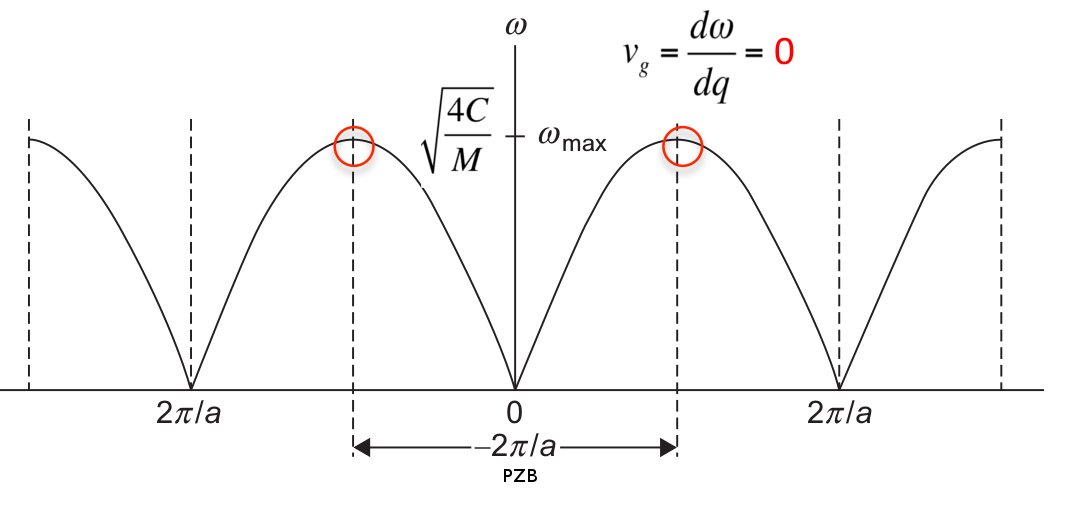
\includegraphics[width=\textwidth]{figures/reldisp.png}
  \caption{Relación de dispersión para la cadena lineal
    monoatómica. Notar como es periódica fuera de la primera zona de
    Brillouin.}
  \label{fig:reldisp}
\end{figure}

Para longitudes de onda largas ($qa l 1$) recupero la aproximación a
medio continuo, y la relación de dispersión es lineal:
\begin{equation}
  \omega(q l) \sim \sqrt{ \frac{C}{M}}aq \propto q
\end{equation}

En los límites de la primera zona de Brillouin ($\pm \frac{\pi}{a}$),
la relación de dispersión se aplana y por tanto $v_g =
\frac{\text{d}\omega}{\text{d}q} = 0$.

La máxima longitud de onda posible es $\lambda_{\text{min}} =
\frac{2\pi}{q_{\text{max}}} = 2a$.

\section{Cadena diatómica}
Ahora supongamos que la cadena tiene, de forma alternada, dos masas
$M_1 > M_2$. Llamamos $a$ a la distancia entre dos masas iguales (la
situación es como en la cadena monoatómica pero con una base
doble). Siendo $C$ la constante de acoplamiento de todos los
``muelles'', y $u,v$ las posiciones de las masas $M_1, M_2$:
\begin{equation}
  \begin{cases}
    M_1 \ddot u_s &= C [V_s + V_{s-1} - 2u_s] \\
    M_2 \ddot v_s &= C [u_{s+1} + u_{s} - 2v_s]
  \end{cases}
\end{equation}
Volviendo a probar con soluciones de tipo periódico, se obtiene
\begin{equation}
  \begin{pmatrix}
    -\omega^2M_2 + 2C && -C(1+e^{-iqa}) \\
    -C(1+e^{iqa}) && -\omega^2M_1 + 2C
  \end{pmatrix}
  \begin{pmatrix}
    u_0 \\ v_0
  \end{pmatrix} = 0
\end{equation}
Para que haya soluciones, el determinante de la matriz ha de ser
nulo. Imponiendo esa condición, se obtienen dos relaciones de
dispersión, correspondientes a dos ramas (fig. \ref{fig:twobranches}):
\begin{equation}
  \omega^2 = \frac{C(M_1+M_2)}{M_1M_2} \left[ 1 \pm \sqrt {1 - \frac{4
      M_1M_2}{(M_1M_2)^2}\sin^2qa} \right]
\end{equation}
\begin{figure}
  \centering
  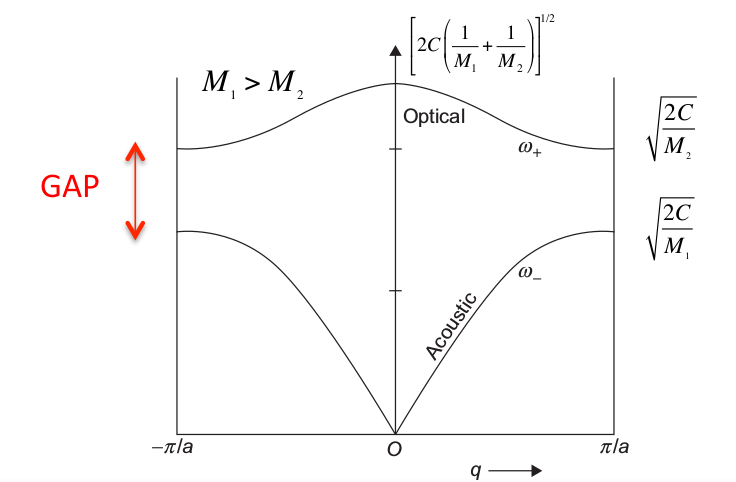
\includegraphics[width=\textwidth]{figures/twobranches.png}
  \caption{Al tener una base con más de un átomo, aparece una nueva
    rama en la relación de dispersión.}
  \label{fig:twobranches}
\end{figure}

\section{Caso 3D}
En 3D, para una base de $r$ átomos, hay $3r$ ramas; 3 acústicas
(2 transversales y una longitudinal) y $3r-3$ ópticas. Veamos la
ecuación que las define.

Sea un átomo $\alpha$ en una celda unidad
(fig. \ref{fig:3dmodesdiagram}), $\phi = \phi(\{\mathbf{r}_{n\alpha} +
\mathbf{u}_{n\alpha}\})$. Supongo que los posibles
desplazamientos son muy pequeños ($\mathbf{u}_{n\alpha} l$) y efectúo
un desarrollo en serie de Taylor.
\begin{equation}
\begin{split}
  \phi &\sim
  \underbrace{\phi(\{\mathbf{r}_{n\alpha}\})}_{\text{cohesión}} +
  \sum_{n,\alpha,i} \left[  \frac{\partial \phi}{\partial
      r_{n,\alpha,i}}\right] _0 u_{n,\alpha, i} + \\ &+ \frac{1}{2}
  \sum_{n,\alpha,i} \sum_{n,\beta,j} \left[  \frac{\partial ^2
      \phi}{\partial r_{n,\alpha,i} \partial r_{n,\beta,j}}\right]_0
  u_{n,\alpha,i} u_{n,\beta,j} + \cdots
\end{split}
\end{equation}
donde $\alpha, \beta \in \{1, \cdots, r\}$ recorren todos los átomos de la celda unidad,
$n \in \{ 1, \cdots , N\}$ cada índice de celda en toda la red e $i,j \in \{ \hat x, \hat y, \hat z \}$ las 3 coordenadas x,y,z.

El segundo término es nulo, ya que se evalúa en la posición de
equilibrio, y nos quedamos en aproximación armónica (orden 2). Esto
nos eliminará algunos efectos anharmónicos, como la expansión térmica.

Defino las \emph{constantes de acoplamiento}
$\phi_{n\alpha i}^{m\beta j} =\left[ \frac{\partial ^2 \phi}{\partial
    r_{n,\alpha,i} \partial r_{n,\beta,j}}\right]_0 $.
Con esta definición, $\phi_{n\alpha i}^{m\beta j} u_{m\beta j}$ es la
fuerza en el átomo $\alpha$ de la celda $n$ en la dirección del espacio
$i \in \{ \hat x, \hat y, \hat z \}$ cuando desplace el átomo $\beta$
de la celda $m$ en la dirección $j\in \{ \hat x, \hat y, \hat z \}$
una cantidad $u$. Poseen algunas características particulares:
\begin{itemize}
\item Invariancia traslacional: $\phi_{n\alpha i}^{m\beta j} = \phi_{0\alpha i}^{(m-n)\beta j} $
\item Son reales
\item Son simétricas, $\phi_{n\alpha i}^{m\beta j} =\phi^{n\alpha i}_{m\beta j} $
\item $ \sum _{m\beta j }\phi_{n\alpha i}^{m\beta j}  = 0$
\end{itemize}
\begin{figure}
  \centering
  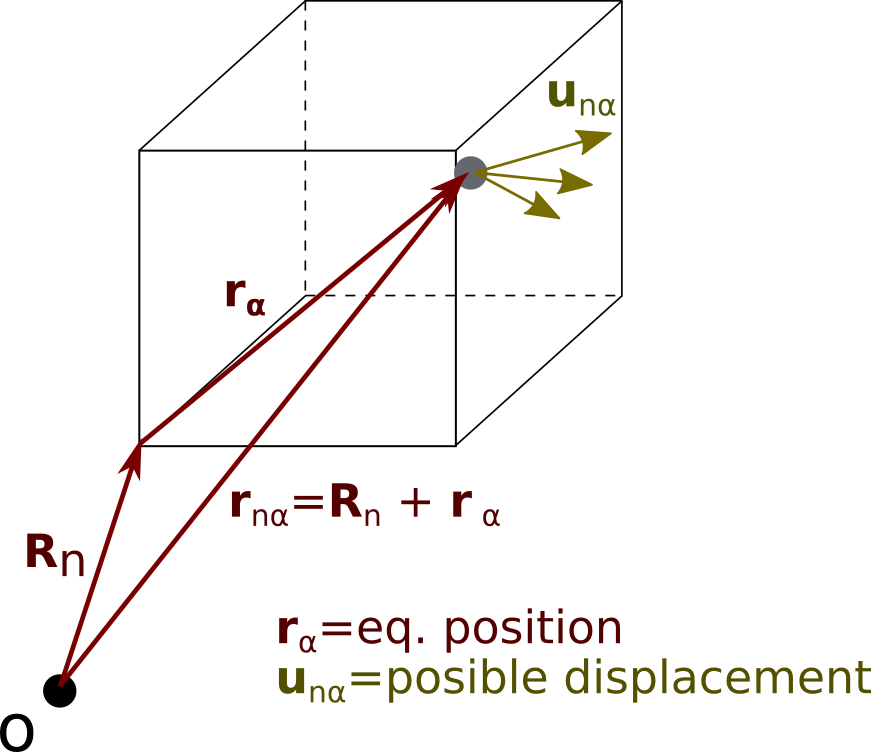
\includegraphics[width=0.5\textwidth]{figures/3dmodesdiagram.png}
  \caption{Geometría en 3D.}
  \label{fig:3dmodesdiagram}
\end{figure}


Las ecuaciones del movimiento para el átomo $\alpha$ de la celda $n$
en dirección $i$ son el siguiente sistema de  $3Nr$ ecuaciones
diferenciales acopladas:
\begin{equation}
  M_\alpha \ddot u_{n\alpha i} + \sum_{m\beta j} \phi_{n\alpha i
  }^{m\beta j} u _{m\beta j} = 0
\end{equation}

Para resolverlas, utilizo un ansatz:
\begin{equation}
  u_{n\alpha i } = \frac{1}{\sqrt M_\alpha} u_{\alpha i} (\mathbf{q})
  e^{i(\mathbf{q}\mathbf{R}_n - \omega t)}
\end{equation}
Y obtengo
\begin{equation}
  -\omega^2 u_{\alpha i} (\mathbf{q}) + \frac{1}{\sqrt{M_\alpha
      M_\beta}}\sum_{m\beta j} \phi _{n\alpha i}^{m\beta j }u_{\beta j
  }(\mathbf{q}) e^{i \mathbf{q}(\mathbf{R}_m -\mathbf{R}_n )} = 0
\end{equation}
Defino la matriz dinámica. No es más que la transformada de Fourier de
las constantes de acoplamiento, o la matriz de éstas en el espacio recíproco.
\begin{equation}
\begin{split}
 D_{\alpha i }^{\beta j} &= \frac{1}{\sqrt{M_\alpha
      M_\beta}} \sum_{m\beta j} \phi _{n\alpha i}^{m\beta j } e^{i
    \mathbf{q}(\mathbf{R}_m -\mathbf{R}_n )} \\
&= \frac{1}{\sqrt{M_\alpha
      M_\beta}} \sum_{p} \phi _{0\alpha i}^{p\beta j } e^{i
    \mathbf{q}(\mathbf{R}_p)}
\end{split}
\end{equation}
Posee ciertas propiedades, que nos dan información sobre las $\omega$:
\begin{itemize}
\item Si las $\phi$ son reales, la matriz es hermítica. Por tanto, las
  $\omega^2$ son reales.
\item Es periódica ante desplazamientos en la red recíproca, $\tilde D
  (\mathbf{q}) = \tilde D (\mathbf{q} + \mathbf{G})$. Esto implica que
  $\omega$ también.
\item Es invariante bajo inversión temporal. Si cambiamos de $t$ a
  $-t$, cambiamos de $q$ a $-q$, y tenemos que $\tilde D (\mathbf{q})
  = \tilde D (\mathbf{-q})$, y por tanto $\omega (\mathbf{q}) = \omega (\mathbf{-q})$.
\end{itemize}
Con ella, el sistema se puede expresar de manera más compacta como
\begin{equation}
  \boxed{
    -\omega^2 u_{\alpha i} (\mathbf{q}) + \sum_{\beta j} D_{\alpha
      i}^{\beta j} u_{\beta j} = 0
  }
\end{equation}
Se puede llegar a una ecuación de autovalores en poniendo la ecuación
como $\sum_{\beta j} \left[ D_{\alpha i}^{\beta j} (\mathbf{q})  -
  \omega^2 \delta_{\alpha i }^{\beta j}\right] u_{\beta j} (
\mathbf{q}) = 0$:
\begin{equation}
  | \tilde D ( \mathbf{q}) - \omega^2 \mathbb{I} | = 0
\end{equation}
Esta ecuación de autovalores para la matriz dinámica nos da $3r$
soluciones; $3$ son ramas acústicas y $3n - 3$ ópticas.

\section{Modelo cuántico}

\subsection{Cadena lineal monoatómica}
Definimos el hamiltoniano del sistema:
\begin{equation}
  \mathcal{H} = \sum_{n=1}^{N} \frac{p_n^2}{2M} + \frac{1}{2} C
  \sum_{n=1}^{N} (u_{n+1} - u_n)^2
\end{equation}
Como estamos bajo el modelo de la física cuántica $u$ y $p$ son
operadores, y $[u_n, p_{n'}] = i \hbar \delta_n^{n'}$. Para resolver
el sistema tomamos los siguientes pasos:
\begin{itemize}
\item Pasamos a coordenadas normales los operadores, trabajamos en el
espacio de las $\mathbf{q}$ de los fonones.
\item Hacemos las cuentas.
\item Definimos los operadores de creación y destrucción.
\end{itemize}
Definimos los operadores de coordenadas normales $Q$ y $P$:
\begin{equation}
  \begin{cases}
    Q_q = \frac{1}{\sqrt N} \sum_{n}^{ } u_n e^{-iqna} \\
    P_q = \frac{1}{\sqrt N} \sum_{n}^{ } p_n e^{iqna}
  \end{cases} \rightarrow
  \begin{cases}
    u_n = \frac{1}{\sqrt N} \sum_{q}^{ } Q_q e^{iqna} \\
    p_n = \frac{1}{\sqrt N} \sum_{q}^{ } P_q e^{-iqna}
  \end{cases}
\end{equation}
Estos operadores satisfacen la relación de conmutación, y son
operadores de posición y momento:
\begin{equation}
  [Q_q, P_{q'}] = \frac{1}{N}  \underbrace{\sum_{n,n'}^{ }[u_n,
    p_{n'}]}_{= 0 + 0 + \cdots + 1 + 0 + \cdots + 0} e^{-iqna}
  e^{iqn'a} = \frac{1}{N}i \hbar 1 \sum_n e^{i(q-q')na} = i \hbar \delta_q^{q'}
\end{equation}
Notar que la última suma resulta $N\delta_q^{q'}$ por ser una suma de
red (ver apéndice \ref{chap:latticesum}). Bastaría cualquier vector de
la red recíproca, pero $\mathbf{G} = 0$ es el único en primera zona de
Brillouin.

\section*{Valores permitidos de $q$}
Supongamos una cadena finita, esto nos introducirá una restricción en
$q$ que no existía en el caso previamente considerado. Impongamos unas condiciones de
contorno, la cual no será determinante en tamaños grandes. En este
caso utilizaremos condiciones periódicas:
\begin{equation}
  u_n = u_{n+N} \rightarrow e^{iqNa} = 1 \rightarrow \boxed{ q =
    \frac{2\pi n}{Na}}
\end{equation}
Tenemos por tanto un espectro finito y discreto para $q$.
No es infinito, ya que nos restringimos a primera zona de Brillouin:
\begin{equation}
  q_{\text{max}} = \frac{\pi}{a} \ \rightarrow \ n_{\text{max}}  = \frac{N}{a}
\end{equation}
Por tanto, $q \in \left[\frac{-\pi}{a}, \frac{\pi}{a}\right]$ y $n \in
\left[\frac{-N}{2}, \frac{N}{2}\right]$.

\section*{Sustitución en $\mathcal{H}$}
Sustituimos en $\mathcal{H}$ los operadores $Q$ y $P$. Aparecen
algunas sumas de red, que crean deltas de Dirac.
\begin{equation}
\begin{split}
  \sum_n \frac{p^2}{2M} &= \frac{1}{2M}  \frac{1}{\sqrt
    N}\sum_{q,q'}^{ } p_q p_q' \sum_{n}^{ } e^{-i(q-q')na} =\\ &= \frac{1}{2M}  \frac{1}{\sqrt
    N}\sum_{q,q'}^{ } p_q p_q' ( N\delta_q^{-q'} ) = \frac{1}{2M} \sum_{q,q'}^{ } p_q p_{-q}
\end{split}
\end{equation}
De manera análoga,
\begin{equation}
  \frac{1}{2} C \sum_{n}^{ } (u_{n+1} - u_n)^2 = \cdots = \frac{1}{2}
  C \sum_{q}^{ } Q_q Q_{-q} (e^{iqn} - 1) (e^{-iqn} - 1) = \cdots
\end{equation}
Como $(e^{iqn} - 1) (e^{-iqn} - 1) = 2 (1 - \cos qa) = \frac{M
  \omega^2 (q)}{C}$, concluimos
\begin{equation}
  \cdots = \frac{M}{2} \sum_q Q_q Q_{-q} \omega^2 (q)
\end{equation}

En coordenadas normales, nos queda una $\mathcal{H}$ desacoplada:
\begin{equation}
  \boxed{
    \mathcal{H}_{\text{norm}} = \sum_{q}^{ } \left[ \frac{1}{2M} P_q
      P_{-q} + \frac{1}{2} M \omega^2 (q) Q_q Q_{-q} \right]
}
\end{equation}

\section*{Operadores de creación y destrucción}
Su definición es similar a la del oscilador armónico:
\begin{equation}
  Q_q = \sqrt{\frac{\hbar}{2M\omega (q)}} (a_q + a^\dagger_{-q})
\end{equation}
\begin{equation}
  P_q = \frac{i\hbar}{2} \sqrt{ \frac{2M \omega (q)}{\hbar} }
  (a_q^\dagger - a_q)
\end{equation}
Despejando los operadores explícitamente:
\begin{equation}
  a_q = \sqrt{\frac{M\omega}{2\hbar}}Q_q + \frac{i}{\hbar}
  \sqrt{\frac{\hbar}{2M\omega}} P_{-q}
\end{equation}

\begin{equation}
  a^\dagger_q = \sqrt{\frac{M\omega}{2\hbar}}Q_{-q} - \frac{i}{\hbar}
  \sqrt{\frac{\hbar}{2M\omega}} P_{q}
\end{equation}
Recordar que no son hermíticos, pero $aa^\dagger$ sí. Su conmutador es
$[a_q,a_{q'}^\dagger] = \delta_q^{q'}$.


\section*{Resolución del hamiltoniano}
Con los nuevos operadores, se obtiene el hamiltoniano como
\begin{equation}
  \mathcal{H}_\text{norm} = \cdots = \sum_{q}^{ } \hbar \omega(q)
  \left( a_q^\dagger a_q + \frac{1}{2} \right)
\end{equation}
Es el hamiltoniano de una suma de osciladores armónicos
unidimensionales, cada uno con frecuencia $\omega(q)$.

Al cuanto de vibración $\hbar \omega(q)$ lo llamamos
\emph{fonón}. Cada fonón viene indexado por $q$ así que se define de
manera natural $\hbar q$ como el \emph{cuasimomento} del fonón. No se
denota momento ya que los fonones son \emph{cuasipartículas}, no
partículas ``reales''. Al interaccionar con fotones, electrones,
etc. se comporta como si tuviera dicho momento.

Demostremos en segunda cuantización que su momento real es nulo. Sea
$P_\text{total}$ el operador momento total de la excitación colectiva
del sólido:
\begin{equation}
\begin{split}
  P_\text{total} &= \sum_{q}^{ } P_n = \frac{1}{\sqrt N} \sum_{n}^{ }
  \sum_{q}^{ } P_q e^{-iqna} =  \\ &= \frac{1}{\sqrt N} \sum_{n}^{ }
  \sum_{q}^{ } e^{-iqna} \frac{i\hbar}{2} \sqrt{ \frac{2M \omega
      (q)}{\hbar}} (a_q^\dagger - a_{-q}) \\
  \langle P_\text{total} \rangle &\propto \langle n_q | a_q^\dagger - a_{-q} |n_q  \rangle = 0
\end{split}
\end{equation}
\section{Técnicas experimentales}
Las energías toman valores desde el \si{\milli\eV} hasta los \SI{100}{\milli\eV}. La sonda
por excelencia, para scattering inelástico, son los neutrones
térmicos, pero hay más variedad:
\begin{description}
\item[Rayos X] Su energía ronda los \SI{10}{\kilo\eV}, con anchura
  típico de $\sim \SI{1}{\eV}$. Al tener los fonones energías del
  orden del \si{\milli\eV}, tengo que resolver con precisiones de
  $\displaystyle \frac{\SI{10}{\milli\eV}}{\SI{10}{\kilo\eV}} =
  10^{-6}$. Hay que monocromatizar muchísimo, y el cristal ha de ser
  muy bueno, ya que $\Delta \lambda \propto \Delta d$.

  Es posible utilizarlos sólo si se posee un sincrotrón.
\item[Luz visible] No puede hacer gran cosa como sonda ya que de
  $\lambda \sim \SI{6000}{\angstrom}$ obtenemos $k =
  \frac{2\pi}{\lambda} \sim \SI{10e-3}{\per\angstrom}$. Como la primera
  zona de Brillouin es de aproximadamente \SI{1}{\per\angstrom} sólo
  podemos escanear una parte muy pequeña (su origen, en que $q \sim 0$).

  En las ramas ópticas a este scattering se le llama \emph{scattering
    Raman}, en las acústicas \emph{scattering Brillouin}. Son técnicas
  muy complicadas experimentalmente.
\item[Infrarrojos] Ocurre lo mismo que con la luz visible, pero la
  absorción es al menos muy buena por parte de la muestra.
\end{description}

Una vez decidida la sonda, hay que realizar el experimento de
scattering. Su amplitud vendrá gobernada por la siguiente ecuación (similar a la
ecuación \ref{eq:samplitude}, en que se halla la función de Born,
básicamente la amplitud de la onda dispersada):

\begin{equation}
  A \propto e^{-i\omega_0 t} \sum_{\mathbf{R}}^{ }
  e^{-i(\mathbf{k'}-\mathbf{k})\mathbf{R}} \iiint_\text{cell}
  \text{d}\mathbf{x} e^{-i(\mathbf{k'} -\mathbf{k})\mathbf{x}} V(\mathbf{x})\propto \cdots
\end{equation}
Recordar que utilizamos $k$ para fotones y $q$ para fonones. Por
sencillez, $r=1$. Se excita un fonón con $\mathbf{q}$ y
$\omega(\mathbf{q})$:
\begin{equation}
  \mathbf{x} = \mathbf{u}(t) = \mathbf{u}_0 e^{\pm i
    (\mathbf{q}\mathbf{R} - \omega t)}
\end{equation}
Utilizando un análisis similar al de la sección
\ref{subsec:formfactor} podemos transformar la integral en una
exponencial, salvo por el factor de forma que absorbemos en el
prefactor de resolución experimental etc. Obtenemos:

\begin{equation}
\begin{split}
  \cdots &\propto e^{-\omega_0 t}\sum_{\mathbf{R}}^{} e^{-i (\mathbf{k'} -
    \mathbf{k}) \mathbf{R}}  \underbrace{e^{-i(\mathbf{k'} - \mathbf{k}) \mathbf{u}}
}_{\sim 1 - i(\mathbf{k'} - \mathbf{k} ) \mathbf{u}} = \\
&= \underbrace{e^{-i\omega_0 t}\sum_{\mathbf{R}}^{ }e^{-i(\mathbf{k'}-
  \mathbf{k}) \mathbf{R}}}_{\text{elastic part}} + \underbrace{-i(\mathbf{k'}-
  \mathbf{k}) e^{-i\omega_0 t} \sum_{\mathbf{R}}^{ } e^{-i
  (\mathbf{k'} - \mathbf{k}) \mathbf{R}} \cdot \mathbf{u}_0 e^{\pm i
  (\mathbf{q} \mathbf{R} - \omega t)}}_{\text{inelastic part}}
\end{split}
\end{equation}

Analicemos la parte inelástica:
\begin{equation}
\begin{split}
  A_\text{inelastic} &= -i(\mathbf{k'} - \mathbf{k}) \mathbf{u_0}
  e^{-i\omega_0 t} e^{\mp i \omega t } \sum_{\mathbf{R}}^{ } e^{-i
    (\mathbf{k'} - \mathbf{k})\mathbf{R}} e^{\pm i
                       \mathbf{q}\mathbf{R}} = \\
                     &= -i(\mathbf{k'} - \mathbf{k}) \mathbf{u_0}
  \exp( {-i \underbrace{(\omega_0 \pm \omega)}_{\omega_f}t} )  \sum_{\mathbf{R}}^{ } e^{-i
    [(\mathbf{k'} - \mathbf{k}) \mp \mathbf{q}]\mathbf{R}}
\end{split}
\end{equation}

El proceso es similar a una colisión clásica (fig. \ref{fig:stokes}), tenemos una ley de
conservación de la energía y otra de conservación del momento:
\begin{itemize}
\item La ley de conservación de la energía es simplemente $\hbar
  \omega_f = \hbar \omega_0 \pm \hbar \omega$.
\item La suma de red me da una condición extra para no anularse, que
  será nuestra conservación del ``momento'':
  \begin{equation}
    \sum_{\mathbf{R}}^{ } e^{-i [(\mathbf{k'} - \mathbf{k}) \mp
      \mathbf{q}]\mathbf{R}} = \delta_{(\mathbf{k'}- \mathbf{k}) \mp
      \mathbf{q}}^\mathbf{G} \rightarrow \mathbf{k'} - \mathbf{k} \mp
    \mathbf{q} = \mathbf{G}
  \end{equation}
  Por tanto $\hbar \mathbf{k'} - \hbar \mathbf{k} \mp \hbar \mathbf{q}
  = \hbar \mathbf{G}$.
\end{itemize}

Si el signo de $\omega_0 \pm \omega$ se toma positivo, se tiene
$\omega_f = \omega_0 + \omega$, la absorción de un fonón. Se denota
\emph{proceso anti-Stokes}. Las leyes quedan como
\begin{itemize}
\item $\hbar \omega_f =
\hbar \omega_0 + \hbar \omega(q)$
\item $\hbar \mathbf{k'} = \hbar
\mathbf{k} + \hbar \mathbf{q} + \hbar \mathbf{G}$
\end{itemize}

Si el signo de $\omega_0 \pm \omega$ se toma negativo, se tiene
$\omega_f = \omega_0 - \omega(q)$, la absorción de un fonón. Se denota
\emph{proceso Stokes}. Las leyes quedan como
\begin{itemize}
\item $\hbar \omega_f =
\hbar \omega_0 - \hbar \omega(q)$
\item $\hbar \mathbf{k'} = \hbar
\mathbf{k} - \hbar \mathbf{q} + \hbar \mathbf{G}$
\end{itemize}

\begin{figure}
  \centering
  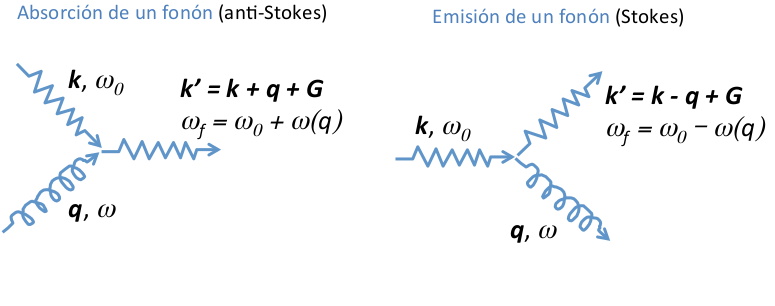
\includegraphics[width=0.8\textwidth]{figures/stokes.png}
  \caption{Procesos de emisión y absorción de fonones ($\leadsto$) por fotones ($\rightsquigarrow$).}
  \label{fig:stokes}
\end{figure}



Los procesos con $\mathbf{G} = \mathbf{0}$ se denotan procesos
normales o procesos N, si $\mathbf{G} \neq \mathbf{0}$ se denotan
procesos \emph{Umklapp} o procesos U.




\chapter{Propiedades térmicas de la red}

Comenzamos el análisis por el caso de una cadena lineal, para luego
pasar al caso 3D. La cadena es finita (con $N$ partículas). Es
absolutamente imprescindible poner condiciones de contorno, pero su
elección sólo se notará en cadenas cortas, siendo irrelevante para $N$ grande.

Utilicemos condiciones de contorno periódicas (Born-Von Karman). Como
ya vimos implican que $e^{iqNa}=1$, y por tanto
$q = \frac{2\pi n}{Na}$. Que $q\in \text{PZB}$ implica que
$q\cdot a \in [-\pi, \pi]$ y por tanto
$n \in \left[ \frac{-N}{2}, \frac{N}{2} \right]$. La densidad de
estados en $q$ es
\begin{equation}
  D(q) = \frac{\text{d}N}{\text{d}q} \sim \frac{\Delta N = 1}{\Delta q}= \frac{1}{2\pi / Na} = \frac{Na}{2\pi}
\end{equation}
Para $\omega$, conocido que $\omega(q) = \omega_\text{max} \lvert \sin
\frac{qa}{2}\vert$, tenemos
\begin{equation}
\begin{split}
  D(\omega) &= \frac{\text{d}N}{\text{d}\omega} = 2
  \frac{\text{d}N}{\text{d}q}
  \frac{1}{\frac{\text{d}\omega}{\text{d}q} = v_g} =\\
            &= 2 \frac{Na}{2\pi}\frac{1}{v_g = \cdots =
  \frac{a}{2}(\omega_\text{max}^2 - \omega^2)^{1/2}} = \\
            &= \frac{2N}{\pi} \frac{1}{\sqrt{\omega_\text{max}^2 - \omega^2}}
\end{split}
\end{equation}
Con $v_g$ calculado por magia negra\footnote{Si escribes
$\frac{\text{d}\omega(q)}{\text{d}q} = \frac{a}{2}(\omega_\text{max}^2
- \omega^2)$ con $\omega(q) = \omega_\text{max} |\sin(qa/2)|$ sale.}.  El
2 surge al contemplar que existen dos $q$ distintas en cada $\omega$, ya
que $q$ y $-q$ dan la misma $\omega$.

La densidad de estados en función de $\omega$ diverge cuando la
velocidad de grupo es nula, en primera zona de Brillouin. Para
$\omega$ nulo converge a un valor constante $\frac{2N}{\pi \omega_\text{max}}$.

En 3D, la densidad de estados resulta
\begin{equation}
\begin{split}
  D(q) &= \frac{1}{\Delta q} = \frac{1}{\Delta q_1 + \Delta q_2 +
    \Delta q_3} = \frac{1}{\frac{2\pi}{N_1 a_1} +  \frac{2\pi}{N_2
      a_2} + \frac{2\pi}{N_3 a_3} } = \\ &= \frac{(N_1 N_2 N_3)(a_1 a_2
         a_3)}{8\pi^3} = \frac{(N_\text{cells})(\Omega)}{8\pi^3} =
                                           \frac{V_\text{cristal}}{8\pi^3}
                                           = \text{cte.}
\end{split}
\end{equation}
El resultado era previsible, ya que
$D(q) =\frac{\text{Number of q's}}{\Omega_q^\text{PZB}} =
\frac{N}{(2\pi)^3/ \Omega} = \frac{N\Omega}{8\pi^3} =
\frac{V_\text{cristal}}{8\pi^3}$.

Una vez conocida la densidad de estados, podemos convertir las sumas
sobre las $\mathbf{q}$ en integrales, quedando estas como
\begin{equation}
  \sum_{\mathbf{q}\in \text{PZB}} f = \int D(\mathbf{q}) f \text{d}\mathbf{q} =
  \frac{V}{8\pi^3}\int f \text{d}\mathbf{q}
\end{equation}

Si tenemos una función de $\omega$ en lugar de $\mathbf{q}$, se
necesita la $D(\boldsymbol{\omega})$ tridimensional. Para hallarla,
imaginamos en el espacio de las $\mathbf{q}$ las superficies
$\omega = \text{cte.}$ y $\omega +
\text{d}\omega = \text{cte.}$ (fig. \ref{fig:wsurface}).


El volumen entre ambas superficies es el número de modos entre
$\omega$ y $\omega + \text{d}\omega$, $D(\omega) \text{d}\omega$, y será:
\begin{equation}
  D(\omega) \text{d} \omega = \frac{V}{8\pi^3} \iint_{\partial
    S_\omega} \underbrace{\text{d}S_\omega \text{d}q_\perp}_{\mathbf{q}} = \cdots
\end{equation}
Como $d\omega = |\nabla_\mathbf{q}
\omega(\mathbf{q})|\text{d}q_\perp$, obtenemos al despejar para
$\text{d}q_\perp$:
\begin{equation}
 \cdots = \frac{V}{8\pi^3} \iint_{\partial S_\omega} \text{d}S_\omega \frac{\text{d}\omega}{|\nabla_\mathbf{q}\omega(\mathbf{q})|}
\end{equation}
Por tanto, identificando $\nabla_\mathbf{q} \omega(\mathbf{q})$ con la
velocidad de grupo,
\begin{equation}
  D(\omega) \text{d}\omega = \frac{V}{8\pi^3}  \text{d}\omega \iint_{\partial
    S_\omega} \frac{\text{d}S_\omega}{v_g}
\end{equation}

\begin{figure}
  \centering
  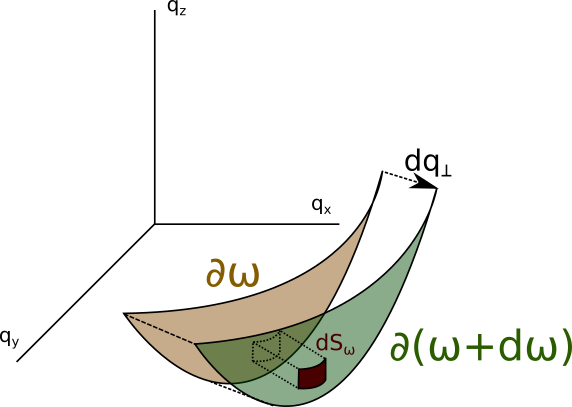
\includegraphics[width=0.6\textwidth]{figures/wsurface.png}
  \caption{Se muestra un corte de la zona entre las superficies
    $\omega = \text{cte.}$ y $\omega + \text{d}\omega= \text{cte.}$}
  \label{fig:wsurface}
\end{figure}

Notar como la densidad de estados en $\omega$ diverge cuando la
velocidad de grupo se anula (en el caso 1D ocurría en la frontera con
la primera zona de Brillouin). A estos picos se les denota
\emph{singularidades de Van Hove}.

El resultado hallado con el análisis de las superficies $\omega =
\text{cte.}$ es general y vale para otros casos, como los electrones.

\section{Calor específico de la red}
\label{sec:cvlattice}
El calor específico a volumen constante será
\begin{equation}
  c_v = \left( \frac{\partial U}{\partial T} \right)_V
\end{equation}
Se puede relacionar con el calor específico a presión constante con la
relación experimental $c_p - c_v = 9 \alpha^2 B V^2 T$, donde $\alpha$
es el coeficiente de dilatación térmica y $B$ el módulo de
compresibilidad. En aproximación armónica, como se demostrará a
continuación, $\alpha = 0$ y $c_v = c_p$.

Para los fonones se tiene que $E = \sum_{q,\lambda}^{ }(n_{q,\lambda} +
1/2) \hbar \omega_\lambda (q)$, donde $\lambda$ son las distintas
ramas de fonones. Por tanto, en el sólido,
\begin{equation}
\label{eq:phU}
  U = \langle E \rangle + U_\text{eq} =  \sum_{q,\lambda}^{
  }(\langle n_{q,\lambda} \rangle + 1/2) \hbar \omega_\lambda (q) + U_\text{eq}
\end{equation}
Al ser bosones siguen una distribución de Bose-Einstein con $\mu = 0$,
luego $\langle n_{q,\lambda} \rangle= \left[\exp(\frac{\hbar \omega_\lambda
  (q)}{\kb  T}) - 1\right]^{-1}$ y por tanto el calor específico es (a
volumen constante):
\begin{equation}
\label{eq:phc}
  c_{\text{phonons}} = \left( \frac{\partial U}{\partial T} \right)_V
  = \cdots = \kb  \sum_{q,\lambda}^{} x^2 \frac{e^x}{(e^x-1)^2}, \ \ x = \frac{\hbar
    \omega_{q,\lambda}}{\kb  T}
\end{equation}

Si conozco las $\omega_{q,\lambda}$ puedo resolver $c_\text{ph}$
numéricamente. Cuando $\kb T \gg \hbar \omega_{q,\lambda}$ la expresión
se reduce a la ley de Dulong-Petit, y resulta
\begin{equation}
  \lim_{T\to \infty}c_\text{ph} = \cdots = \kb  N3r= \text{cte.}
\end{equation}
o $3R \ \si{\joule\per\mol\per\kelvin}$. Recordar que $r$ son los átomos en la
celda unidad.

La forma funcional no es clara, pero con modelos adecuados para
$D(\omega)$ (Debye, Einstein) podemos convertir la suma en integral
utilizando la mecánica estadística.

\subsection{Modelo de Einstein}
Se tiene $\omega_\lambda(q) \equiv \omega_E$, y una densidad de
estados cuya distribución es una delta de Dirac:
\begin{equation}
  D(\omega) = 3Nr\delta(\omega-\omega_E)
\end{equation}

El calor específico es, por tanto (sólo queda un término en el sumatorio):
\begin{equation}
  c_{\text{phonons}} =  \kb  3Nr\left( \frac{\hbar \omega_E}{\kb  T}
  \right)^2 \frac{e^{ \frac{\hbar \omega_E}{\kb  T} }}{\left(e^{
        \frac{\hbar \omega_E}{\kb  T} }-1 \right)^2}
\end{equation}
A temperaturas bajas $c_\text{ph} \to 0$ y a temperaturas altas se
recupera el resultado de la ley de Dulong-Petit
(fig. \ref{fig:cph}). Notar que tiende a cero de forma exponencial, no
con $T^3$ como debiera.

El modelo de Einstein funciona bien con las ramas ópticas porque su
$\omega_\lambda(q) \sim \text{cte.}$ Con las acústicas no es
muy exacto. Escribiéndolo sólo para las ramas ópticas se obtiene:
\begin{equation}
  c_\text{ph}^\text{opt} = \kb  3NR (r-1) F_E \left( \frac{\theta_E}{T} \right)
\end{equation}
donde $\theta_E =\frac{\hbar \omega_E}{\kb }$ es la \emph{temperatura
  de Einstein} y $F_E (x) = x^2 \frac{e^{x}}{(e^{x}-1)^2} $ es la
\emph{función de Einstein}.

Para aproximar correctamente las ramas acústicas utilizamos el modelo
de Debye.

\subsection{Modelo de Debye}
Suponemos que $\omega = vq$, y por tanto
\begin{equation}
\begin{split}
  D(\omega) \text{d}\omega &= \frac{V}{8\pi^3} \text{d}\omega
  \iint_{S_\omega} \frac{\text{d}S_\omega}{v_g = v = \text{cte.}} =
  \frac{V}{8\pi^3 } \text{d}\omega \frac{1}{v} \underbrace{[4\pi
    q^2]}_{\iint \text{d}S_\omega} = \\ &= \frac{V}{8\pi^3 v}\text{d}\omega
  4\pi \left( \frac{\omega}{v} \right)^2 = \frac{V}{2\pi^2 v^3}
  \omega^2 \text{d}\omega
\end{split}
\end{equation}
El problema con la expresión obtenida es que hay infinitos estados. Lo
solucionamos introduciendo a mano una frecuencia de corte $\omega_D$,
y ajustándola para que $\int_0^{\omega_D} = n_\text{states}$. Se
suele definir una única frecuencia de corte para todas las ramas:
\begin{equation}
\int_0^{\omega_D} [ D_L(\omega) + D_T(\omega) ] \text{d}\omega = 3N \ \ \rightarrow \ \ \omega_D = \left(
  \frac{6\pi^2 v_\text{av}^3 N}{V} \right)^\frac{1}{3}
\end{equation}
donde $D_L,D_T$ son las densidades de estados para el modo
longitudinal y los dos modos transversales. $v_\text{av}$ se define
como
\begin{equation}
  \frac{3}{v_\text{av}^3} = \frac{1}{v_L^3} + \frac{2}{v_T^3}
\end{equation}
Ahora estamos en condiciones de escribir la energía como integral:
\begin{equation}
  U = \sum_{q,\lambda}
  \frac{\hbar\omega_{q,\lambda}}{e^{\frac{\hbar\omega_{q,\lambda}}{\kb 
      T}}-1} = \int_0^{\omega_D} \frac{\hbar\omega_{q,\lambda}}{e^{\frac{\hbar\omega_{q,\lambda}}{\kb 
      T}}-1} D(\omega)\text{d}\omega
\end{equation}
donde $D(\omega)\text{d}\omega = D_L(\omega) + D_T (\omega) =
\frac{3V}{2\pi^2 v_\text{av}^3} \omega^2 \text{d}\omega$. La energía
queda, por tanto,
\begin{equation}
  U = 9N\kb  T \left( \frac{T}{\theta} \right)^3 \int_0^{x_D}
  \frac{x^3}{e^{x}- 1} \text{d}x
\end{equation}
con $x = \frac{\hbar \omega}{\kb  T}$ y $\theta =  \frac{\hbar}{\kb } \omega_D= \frac{\hbar
  v_\text{av}}{\kb } \left( \frac{6\pi^2 N}{V} \right)^{1/3}$. El calor
específico es por tanto

\begin{equation}
  c_\text{ph}^\text{acoustic} = 9N\kb  T \left( \frac{T}{\theta} \right)^3 \int_0^{\theta/T}
  \frac{x^4 e^{x}}{(e^{x}- 1)^2} \text{d}x
\end{equation}

A altas temperaturas se recupera la ley de Dulong-Petit, y a bajas
convergemos a cero con $T^3$, como se espera. En la figura
\ref{fig:cph} puede verse la forma funcional.

\begin{figure}
  \centering
  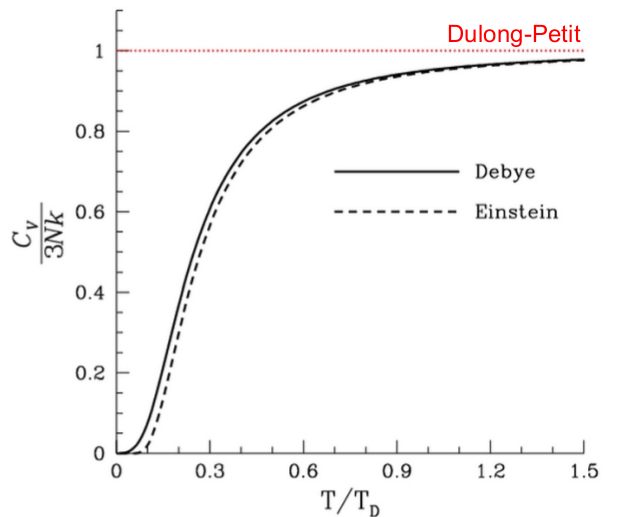
\includegraphics[width=0.8\textwidth]{figures/cph.png}
  \caption{Comparativa de la forma funcional de $c_\text{ph}$ con las
    estadísticas de Einstein y Debye. Notar la discrepancia en el
    orden de la convergencia a cero.}
  \label{fig:cph}
\end{figure}


\section{Dilatación térmica}
La dilatación térmica es un efecto puramente anharmónico, como veremos
a continuación.

Sea el potencial de interacción del sólido
$U(x) = \text{cte.} + cx^2 - gx^3 - fx^4 - \cdots$, con $c,f,g > 0$.
\subsection{Estadística clásica}
La posición media es ($\beta = (\kb  T)^{-1}$):
\begin{equation}
  \langle x \rangle = \frac{\int_\mathbb{R} \text{d}x\  x e^{-\beta
  U(x)}}{ \pazocal{Z} = \int_\mathbb{R} \text{d}x\  e^{-\beta U(x)}} = \cdots
\end{equation}
Si nos quedamos en tercer orden de aproximación,
\begin{equation}
\begin{split}
  \cdots &= \frac{1}{\pazocal{Z}}  \int_\mathbb{R} \text{d}x \ e^{-\beta c x^2}
    e^{\beta(gx^3 + fx^4)} \sim \\ &\stackrel{x \to 0}{\sim}
    \frac{1}{\pazocal{Z}} \int_\mathbb{R} \text{d}x \ x e^{-\beta c
      x^2} (1 + \beta g x^3 + \cancelto{\sim 0}{f x^4}) = \\
         &= \frac{1}{\pazocal{Z}} \beta g\int_\mathbb{R} \text{d}x  \ x^4
           e^{-\beta c x^2} = \frac{3g}{4c^2 } \kb  T
\end{split}
\end{equation}

Por tanto $\alpha$ es
\begin{equation}
  \alpha = \frac{1}{a} \left( \frac{\partial \langle x
      \rangle}{\partial T} \right)_P =  \frac{3g\kb }{4ac^2} = \text{cte.}
\end{equation}
Notar que la aproximación armónica ($g = 0$) resulta en $\alpha =
0$.
Experimentalmente existen ciertas discrepancias; $\alpha =
\alpha(T)$ y
 $\alpha$ puede ser negativa.

Las carencias del modelo se pueden solucionar mediante la aplicación
de la mecánica cuántica\footnote{Cómo no.}.

\subsection{Modelo cuántico (Teoría de Grüneisen)}
Conocemos que
\begin{align}
  \alpha &= \frac{1}{3V} \ppfrac{V}{T}{P} \\
  B &= -V \ppfrac{P}{V}{T}
\end{align}
donde el $3$ en $\alpha$ proviene de considerar un medio isótropo o
cúbico. Ambas expresiones se relacionan mediante
$\alpha = \frac{1}{3B} \ppfrac{P}{T}{V}$. Escribimos la energía libre
de Helmholtz:
\begin{equation}
  F = - \kb  T \log \pazocal{Z} = \sum_{q,\lambda}^{ } \frac{1}{2}
  \hbar \omega_\lambda (q) + \sum_{q,\lambda}^{ } \kb  T \log \left(
    1-e^{-\beta \hbar \omega_\lambda(q)} \right)
\end{equation}
y con ella la presión, notando que la dependencia con el volumen está
en $\omega$:
\begin{equation}
\begin{split}
  P &= - \ppfrac{F}{V}{T} = -\sum_{q, \lambda}^{} \frac{1}{2}
  \frac{\partial}{\partial V}(\hbar \omega_\lambda (q)) -
  \sum_{q,\lambda}^{ }\kb  T \frac{\beta \frac{\partial}{\partial V}
    (\hbar \omega_\lambda (q))}{1-e^{-\beta \hbar\omega_\lambda (q)}}
  \\
    &= - \sum_{q,\lambda}^{ } \left( \langle n_{q,\lambda} \rangle +
      \frac{1}{2}\right) \frac{\partial}{\partial V} (\hbar
      \omega_\lambda (q))
\end{split}
\end{equation}
Para el último paso, se ha identificado
$(1-\exp( 1 -\beta \hbar \omega_\lambda))^{-1}$ como la función de
distribución. Por último, calculamos la derivada de la presión con la
temperatura:
\begin{equation}
  \ppfrac{P}{T}{V} = - \sum_{q,\lambda} \frac{\partial \langle
    n_{q,\lambda}\rangle}{\partial T} \frac{\partial}{\partial V} (
  \hbar \omega_\lambda ( q))
\end{equation}
y por tanto, recordando que $\alpha = \frac{1}{3B} \ppfrac{P}{T}{V}$,
\begin{equation}
  - \sum_{q,\lambda} \frac{\partial \langle
    n_{q,\lambda}\rangle}{\partial T} \frac{\partial}{\partial V} ( \hbar \omega_\lambda ( q)) = 3B \alpha
\end{equation}

Si recordamos las ecuaciones \ref{eq:phU} y \ref{eq:phc}, tenemos que
el calor específico por rama es
$c_\text{ph}^{\lambda(q)} = \frac{1}{V} \hbar \omega_\lambda(q) \frac{\partial
  \langle n_{q,\lambda}\rangle}{\partial T}$, y definiendo el
parámetro $-\gamma_{q,\lambda}$  como
$\frac{V}{\omega_\lambda(q)}\frac{\partial}{\partial V} \omega_\lambda
(q) = - \frac{\partial}{\partial V} \log \omega_\lambda (q)$ se tiene
\begin{equation}
  \alpha = \frac{1}{3B} \sum_{q,\lambda} c_\text{ph}^{\lambda(q)} \gamma_{q,\lambda}
\end{equation}
Definimos el \emph{parámetro de Grüneisen} como
\begin{equation}
  \gamma = \frac{\sum_{q,\lambda} c_\text{ph}^{\lambda(q)}
    \gamma_{q,\lambda}}{c_\text{ph}}
\end{equation}
con valor aproximado entre 1 y 2. El coeficiente de expansión térmica
queda como
\begin{equation}
  \alpha (T)= \frac{\gamma c_\text{ph}}{3B}
\end{equation}
A pesar de que todos los términos dependen de la temperatura la mayor
dependencia está en $c_\text{ph}$, ya que $B \sim \text{cte.}$ y
$\gamma$ oscila entre 1 y 2.


\section{Conductividad térmica}
La ley de Fourier (1807) dicta
\begin{equation}
  \mathbf{J}_Q = - \kappa \nabla T
\end{equation}
donde $\kappa$ es la \emph{conductividad térmica}. Calculémosla para
un aislante eléctrico; en él solo habrá dinámica de red.

\subsection{Teoría cinética elemental}
\label{sec:tce}


Identificamos a los fonones como los portadores de calor en el sólido,
crean la \emph{corriente térmica}. Se descarta que los portadores sean
los electrones por estar considerando un aislante.

Los fonones poseerán un recorrido libre medio $\Lambda$, limitado por
factores intrínsecos (las colisiones entre fonones, efecto
anharmónico) y extrínsecos:
\begin{itemize}
\item Límites geométricos, dados por las dimensiones del cristal.
\item Dispersión de fonones por defectos en el cristal.
\item Dispersión por impurezas.
\end{itemize}

La corriente térmica depende de $\Lambda$ (figura \ref{fig:jcurrent})
a través de la energía de los fonones:
\begin{figure}
  \centering
  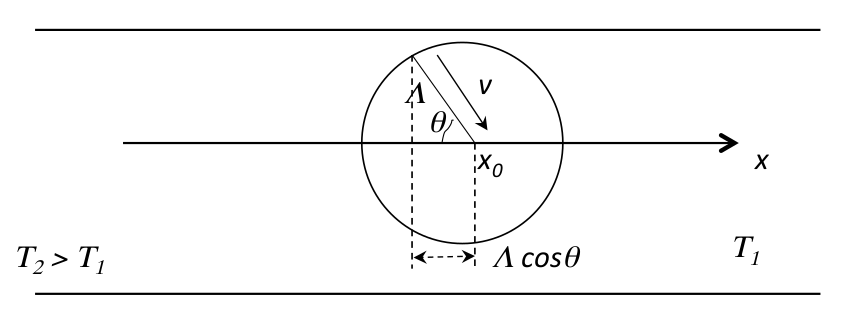
\includegraphics[width=0.8\textwidth]{figures/jcurrent.png}
  \caption{Dispersión de los fonones en una corriente térmica.}
  \label{fig:jcurrent}
\end{figure}

\begin{equation}
  \mathbf{J}_Q \cdot \hat x = \langle
  \underbrace{v_x}_{\mathclap{V_\text{ph}}} \ \ \cdot \ \ \underbrace{u(x_0
  - \Lambda \cos \theta)}_{\mathclap{\text{volume unit energy of
      ph.}}} \ \rangle_\theta = \cdots
\end{equation}
donde el subíndice $\theta$ indica un promediado a todos los
ángulos y $v_x = v\cos \theta$. Integrando a todo el ángulo sólido
($\text{d} \Omega = \text{d}\theta \sin \theta \text{d}\phi$):
\begin{equation}
\begin{split}
  \cdots &= \int_0^{\pi} [v \cos \theta] [u(x_0 - \Lambda \cos \theta)] \frac{2\pi
           \sin \theta \text{d}\theta}{4\pi} = \\
         &=  \frac{v}{2} \int_0^\pi
           \underbrace{\left[ u(x_0) - \Lambda\cos \theta \frac{\partial
           u}{\partial x} \bigg|_{x_0} \right]}_{u(x_0 - \Lambda \cos
           \theta)} \cos \theta \sin \theta \text{d} \theta = \\
         &= \frac{u(x_0)v}{2} \int_0^\pi \sin \theta \cos \theta
           \text{d}\theta - \frac{1}{2} \Lambda v \pfrac{u}{x}{}
           \underbrace{\int_0^\pi \sin \theta \cos^2 \theta
           \text{d}\theta}_{2/3} = \\
         &= -\frac{1}{3} \Lambda v \pfrac{u}{T}{} \pfrac{T}{x}{} =
           \frac{-1}{3} \Lambda v c_v \pfrac{T}{x}{} = -\kappa \nabla T
\end{split}
\end{equation}

Por tanto, $\kappa = \Lambda c_v v / 3$. En función del tiempo de
relajación $\tau$, donde $\Lambda = v \tau$, se tiene
\begin{equation}
  \kappa = \frac{1}{3} v^2 \tau c_v
\end{equation}

\section{Ecuación de fonones de Boltzmann}
La corriente tiene unidades de energía por velocidad, así que de
manera genérica:
\begin{equation}
  \mathbf{J}_Q = \sum_{\mathbf{q}} \langle n(\mathbf{q})\rangle \hbar
  \omega(\mathbf{q}) \mathbf{v} ( \mathbf{q})
\end{equation}
Trabajando en 1D para eliminar vectores,
$j_q = \sum_{\mathbf{q}} \langle n(\mathbf{q})\rangle \hbar
\omega(\mathbf{q}) v_x(\mathbf{q})$.
Es tentativo usar una función de distribución de Bose-Einstein, pero
no estoy en equilibrio (existe un gradiente de temperatura).

En equilibrio, $\langle n(q)\rangle = \langle n(-q)\rangle$, y como
$\omega(q) = \omega(-q)$ y $v(q) = -v (-q)$ se tiene que $j_q^\text{eq} = 0$ al
sumar todas las $q$ y $-q$. Introducimos una corrección de
no-equilibrio a la función de distribución, de forma que $\langle n
=q\rangle = \langle n_0 (q)\rangle + \langle n_1 (q)\rangle$ con
$\langle n_0\rangle$ la función de distribución de equilibrio
(Bose-Einstein). Por tanto:
\begin{equation}
  j_q = \sum_{\mathbf{q}} [ \langle n _\mathbf{q}\rangle_0 + \langle
  n_\mathbf{q}\rangle_1 ] \hbar\omega_\mathbf{q} v_{x,\mathbf{q}}=
  \cancelto{0}{j_q^\text{eq}} + \sum_{\mathbf{q}} \langle n_\mathbf{q}\rangle _1\hbar\omega_\mathbf{q} v_{x,\mathbf{q}}
\end{equation}
El problema ahora es aproximar $\langle n _\mathbf{q}\rangle
_1$. Comienzo por notar que estamos en un proceso estacionario y la
variación temporal de $\langle n \rangle$ es nula:
\begin{equation}
  \label{eq:boltz1}
  \frac{\text{d}\langle n \rangle}{\text{d} t} = \pfrac{\langle n
    \rangle}{t}{}\bigg|_\text{diffusion} + \pfrac{\langle n \rangle}{t
  }{} \bigg|_\text{decay} = 0
\end{equation}

Evaluamos el término de difusión:
\begin{equation}
\begin{split}
  \pfrac{\langle n \rangle}{t} \bigg|_\text{diff} &\sim \frac{\langle n(x - v_x \Delta t
    )\rangle - \langle n (x)\rangle}{\Delta t} \sim \frac{ \langle
                                 n(x)
    \rangle  - v_x \Delta t
    \pfrac{\langle n \rangle}{x} - \langle n (x)\rangle}{\Delta t}
                                 \sim \\
                               &= -v_x \pfrac{\langle n \rangle}{T}
                                 \pfrac{T}{x} \sim -v_x \pfrac{\langle n \rangle_0}{T}
                                 \pfrac{T}{x}
\end{split}
\end{equation}
Paca el término de decaimiento, suponemos una vuelta al equilibrio
exponencial:
\begin{equation}
 \pfrac{\langle n \rangle}{t} \bigg|_{\mathrlap{\text{decay}}} \sim \frac{- \langle
   n \rangle - \langle n \rangle_0}{\tau}
\end{equation}

Volviendo a la ecuación \ref{eq:boltz1}, obtengo:
\begin{equation}
  v_x  \pfrac{\langle n \rangle}{T} \pfrac{T}{x} + \frac{\langle n
    \rangle - \langle n \rangle_0}{\tau} = 0
\end{equation}
Comienzo por linealizar la ecuación,
$\pfrac{\langle n \rangle}{x} \sim \pfrac{\langle n
  \rangle_0}{x}$.
Nos queda una ecuación lineal, con el término que nos interesa
($\langle n \rangle - \langle n \rangle_0$) ya despejado,
$ \langle n \rangle - \langle n \rangle_0 = - v_x \tau \pfrac{\langle
  n \rangle_0}{T} \pfrac{T}{x} $.
Por tanto, volviendo a la corriente térmica, obtenemos
\begin{equation}
  j_q = \sum_{q} \tau \pfrac{\langle n \rangle_0}{T} \pfrac{T}{x}
  \hbar \omega v_x^2
\end{equation}
Si el sólido es isótropo o cúbico, $v_x^2 = v^2 / 3$ y
$j_x = - \frac{1}{3} v^2 \pfrac{T}{x} \tau \sum_{q} \pfrac{\langle n
  \rangle_0}{T}\hbar \omega = - \frac{1}{3} v^2 \tau c_v \pfrac{T}{x}
$, recuperándose la antigua aproximación $\kappa = \frac{-1}{3}v^2
\tau c_v$

\section{Interacción fonón-fonón}
Es un fenómeno anharmónico en que aparecen procesos a 3 fonones, en
que un fonón crea dos o un par se aniquila creando uno. Si uso una
aproximación a mayor orden del hamiltoniano, aparecen procesos a
cuatro fonones, cinco...

De manera similar a la cuantización de la aproximación armónica, se
obtiene $\hbar \omega_i = \hbar \omega_f$ y $\mathbf{q}_i =
\mathbf{q}_f + \mathbf{G}$, con $\mathbf{G}$ nula en procesos umklapp.


La densidad de corriente del gas de fonones será
\begin{equation}
  \mathbf{J}_\text{ph} = \sum_{\mathbf{q}} n_\mathbf{q} \hbar \mathbf{q}
\end{equation}

Imaginemos un proceso a tres fonones, en que el fonón 1 se descompone
en los fonones 2 y 3, de forma que
$\mathbf{q}_1 = \mathbf{q}_2 + \mathbf{q}_3 + \mathbf{G}$. La densidad
de corriente si añadimos estos procesos queda como
\begin{equation}
\begin{split}
  \mathbf{J}_\text{ph}' &= \sum_{\mathclap{\mathbf{q} \neq \mathbf{q}_1,
    \mathbf{q}_2, \mathbf{q}_3}} n_\mathbf{q} \hbar \mathbf{q} +
  (n_1 - 1)\hbar \mathbf{q}_1  + (n_1 + 2)\hbar \mathbf{q}_2 + (n_3 + 1)\hbar \mathbf{q}_3 \\
                       &=  \mathbf{J}_\text{ph} + \hbar(-\mathbf{q}_1 +
                         \mathbf{q}_2 + \mathbf{q}_3 )
\end{split}
\end{equation}
Para procesos N resulta igual a $\mathbf{J}_\text{ph}$ ya que $q_1 =
q_2 + q_3$, y por tanto su
influencia es nula en la corriente. Esto puede entenderse de manera
gráfica pensando en como los fonones de procesos N están limitados a
ir en la dirección del original y los de procesos U pueden ir en
dirección contraria gracias al vector extra $\mathbf{G}$ (figura \ref{fig:UNphonons}). Los que van
en dirección contraria son los que colaboran en la corriente de
fonones, haciendo que la conductividad térmica no diverja (figura \ref{fig:phononcurrent}).

\begin{figure}
  \centering
  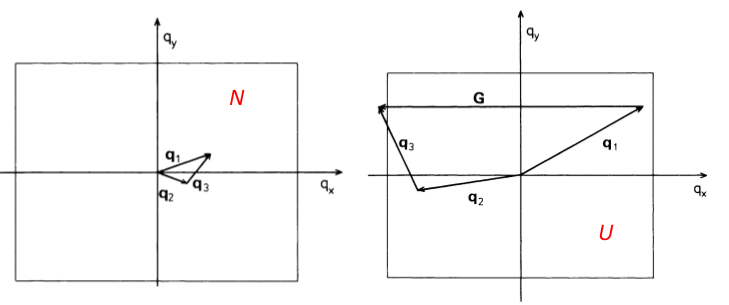
\includegraphics[width=0.8\textwidth]{figures/UNphonons.png}
  \caption{Los fonones de procesos U pueden ir en dirección contraria
    al incidente con el soporte de $\mathbf{G}$.}
  \label{fig:UNphonons}
\end{figure}

\begin{figure}
  \centering
  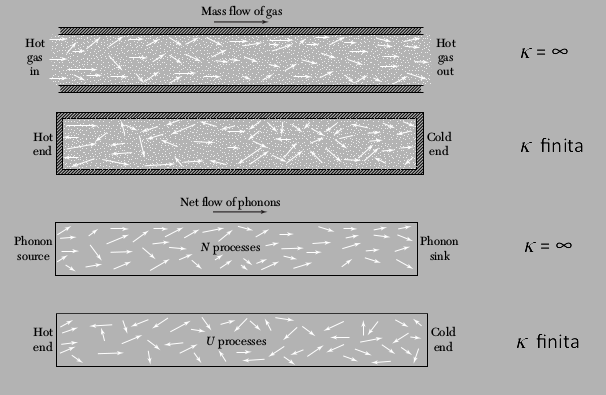
\includegraphics[width=0.8\textwidth]{figures/phononcurrent.png}
  \caption{La conductividad térmica sólo se ve afectada por los
    procesos U. En la analogía de la imagen, se muestra como al igual
    que en los tubos cerrados las paredes generan flujo en dirección
    contraria y limitan la corriente térmica, los fonones de procesos
    U cumplen dicho papel en un sólido.}
  \label{fig:phononcurrent}
\end{figure}

\section{Dependencia térmica de $\boldsymbol{\kappa}$}
\label{sec:ktemp}

Recordamos que $\kappa(T) = \frac{1}{3} v^2 \tau c_v$. En la figura
\ref{fig:thermalk} del apéndice\footnote{En el
    apéndice \ref{app:thermaldep} se analiza con más detalle la
    dependencia térmica.} puede verse la
forma funcional aproximada.

\begin{description}
\item[Altas temperaturas] Para $T \gg \theta_D$ tenemos un calor específico constante, dado por
  la ley de Dulong-Petit. La función de distribución es
  \begin{equation}
    \langle n _q\rangle = \frac{1}{e^{\beta \hbar\omega(q)} -1}
    \stackrel{\beta \to 0}{\sim} \frac{1}{\beta \hbar \omega(q)} =
    \frac{\kb T}{\hbar \omega}
  \end{equation}
  Como $\tau(T) \propto \langle n _q\rangle^{-1}$ (ya que nos importan
  sólo las colisiones fonón-fonón), tenemos que
  $\kappa(T) \propto T^{-1}$.
\item[Bajas temperaturas]
  A temperaturas muy bajas desaparecen muchos fonones y la $\tau$
  divergería si no fuera por contribuciones como la geometría, que la
  llevan a un valor constante. Obtenemos:
  \begin{equation} \kappa \propto c_v \tau \propto T^3 \cdot
    \text{cte.} \propto T^3
  \end{equation}
\end{description}

%%% Local Variables:
%%% mode: latex
%%% TeX-master: "../fesi"
%%% End:
